\section{621 --- Task Scheduler}
Given a char array, $A$, representing tasks CPU need to do. It contains capital letters \texttt{A} to \texttt{Z} where different letters represent different tasks. Tasks could be done without original order. Each task could be done in one interval. For each interval, CPU could finish one task or just be idle.

However, there is a non-negative cooling interval $n$ that means between two same tasks, there must be at least $n$ intervals that CPU are doing different tasks or just be idle.

You need to return the least number of intervals the CPU will take to finish all the given tasks.
 

\paragraph{Example:}

\begin{flushleft}
\textbf{Input}: tasks: $[A, A, A, B, B, B]$, $n = 2$

\textbf{Output}: 8

\textbf{Explanation}: $A \longrightarrow B \longrightarrow \texttt{idle} \longrightarrow A \longrightarrow B \longrightarrow \texttt{idle} \longrightarrow A \longrightarrow B$.

\end{flushleft}
 

\paragraph{Note:}

\begin{itemize}
\item The number of tasks is in the range $[1, 10000]$.
\item The integer $n$ is in the range $[0, 100]$.

\end{itemize}


\subsection{Calculate Idle Slots}
\begin{itemize}
\item If we can get the number of idle slots $x$, the time required to execute all the tasks are $x+z$ where $z$ is the number of total tasks.
\item To find the idle time, take following figure as below ($n=5$):
\begin{figure}[H]
\centering
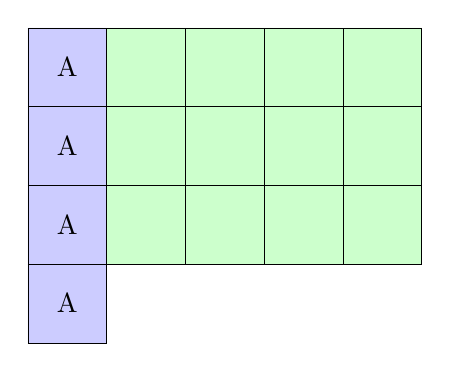
\begin{tikzpicture}
[thick]
\draw[help lines, draw=black, fill=blue!20!] (0,0) grid (1, 4) rectangle (0,0);
\draw[help lines, draw=black, fill=green!20!] (1,1) grid (5, 4) rectangle (1,1);
\node at (0.5, 0.5) {A};
\node at (0.5, 1.5) {A};
\node at (0.5, 2.5) {A};
\node at (0.5, 3.5) {A};
\end{tikzpicture}
\end{figure}
In the figure, the green part represents the idle slots. We can observe that the maximum number of idle slots will always be given by the product of the cooling time and the number of instances of the task with maximum count less 1(in case only multiple instances of the same task need to be executed, and each, then, is executed after lapse of every cooling time). 

The factor of 1 is deducted from the task's count with maximum number of instances, as is clear from the figure, is that in the last round of execution of the tasks, the idle slots need not be considered for insertion following the execution of the related task. 

Now, based on the count of the instances of the other tasks, we can reduce the number of idle slots from this maximum value, to determine the minimum number of idle slots needed.
\item To do that, check the following graph. Assuming the tasks are executed in row-wise order, we can see that in case the number of instances of another task equal the number of instances of the task with maximum number of instances, the number of idle slots saved is equal to its number of instances less 1 as is clear for the case of task B as below. 

\begin{figure}[H]
\centering
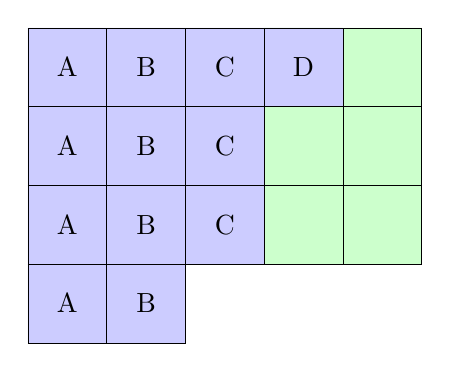
\begin{tikzpicture}
[thick]
\draw[help lines, draw=black, fill=blue!20!] (0,0) grid (1, 4) rectangle (0,0);
\draw[help lines, draw=black, fill=blue!20!] (1,0) grid (2, 4) rectangle (1,0);
\draw[help lines, draw=black, fill=blue!20!] (2,1) grid (3, 4) rectangle (2,1);
\draw[help lines, draw=black, fill=green!20!] (3,1) grid (5, 4) rectangle (3,1);
\node at (0.5, 0.5) {A};
\node at (0.5, 1.5) {A};
\node at (0.5, 2.5) {A};
\node at (0.5, 3.5) {A};

\node at (1.5, 0.5) {B};
\node at (1.5, 1.5) {B};
\node at (1.5, 2.5) {B};
\node at (1.5, 3.5) {B};

\node at (2.5, 1.5) {C};
\node at (2.5, 2.5) {C};
\node at (2.5, 3.5) {C};

\draw[help lines, draw = black, fill=blue!20!] (3,3) grid ++(1,1) rectangle (3,3);
\node at (3.5,3.5) {D};

\end{tikzpicture}
\end{figure}

But, if the count of the number of instances, say $i$ is less than the this maximum value, the number of idle slots saved is equal to the value $i$ itself as is clear for the case of task C. 

Further, for any arbitrary task other than A, B or C with the count of number of instances less than C, such as D. This task can be 
\begin{enumerate}
\item accommodated into the idle slots or 
\item if no more idle slot is available, this task can be appended after every row of tasks without interfering with the cooling time.
\end{enumerate}

In the first case, subtracting its number of instances from the number of idle slots leads to obtaining the correct number of available idle slots. 

In the second case, which will only occur if the number of idle slots pending is already zero, it leads to negative net idle slots, which can later be considered as zero for the purpose of calculations.
\end{itemize}

